
\chapter{Hướng tiếp cận và mô hình đề xuất}
\section{Hướng tiếp cận}

Trong bài toán phân loại hình ảnh hiện hai có hướng tiếp cận chính:
\begin{itemize}
\item Phương pháp thứ nhất: nhận dạng hình ảnh dựa trên tri thức của chuyên gia. Đối với hướng tiếp cận này người ta xây dựng hệ thống phân loại dựa trên các công thức toán học, rút trích đặc trưng của hình ảnh để đưa ra phân loại. Đây là phương pháp truyền thống trước kia, yêu cầu kinh nghiệm của chuyên gia cao, độ chính xác thấp, không thể áp dụng  cho mô hình thay đổi, hay với tập dữ liệu lớn. Tuy nhiên cũng có một số ưu điểm như các công thức tính toán có thể được tính toán dễ dàng, chi phí thấp, không yêu cầu phần cứng cao.
\item Phương pháp thứ hai: nhận dạng hình ảnh dựa trên dữ liệu. Phương pháp này đòi hỏi lượng dữ liệu ban đầu lớn cùng với giải thuật học máy phù hợp để dự đoán, phân loại. Tuy nhiên đối với cách tiếp cận này có thể đảm bảo hệ thống tự động cập nhật các quy tắc nhận dạng mà không cần xây dựng lại công thức tính toán mới. Với sự phát triển công nghệ như hiện nay thì việc thu thập dữ liệu đã không còn là vấn đề nên cách tiếp cận này hiện trở thành hướng tiếp  cận chính trong thị giác máy tính. Chính vì thế đây cũng là hướng mà nhóm sẽ đi theo.
\end{itemize}
%\subsection{ResNet}
%\subsection{Inception}
\section{Công cụ sử dụng}
Cùng với sự phát triển của xử lý ảnh các công cụ phục vụ cũng dần được phát triển trong đó phải kể đến một số framework nổi tiếng như caffe của UC Berkeley, Torch (NYU/Facebook), Theano (U Montreal), TensorFlow (Google),...

Theo định hướng tôi sẽ sử dụng TensorFlow để hiện thực luận văn. Đây là một công cụ mã nguồn mở của Google được hỗ trợ rất mạnh - dễ sử dụng. Hiện tại, cộng đồng hiện sử dụng nó càng được mở rộng.
Ngoài ra còn sử dụng: OpenCV 3.4.4, Keras 2.2.4,...

Một số khái niệm cơ bản cần biết trong TensorFlowt:
\begin{itemize}
\item Scalar : số vô hướng hay các số trong hệ thập phân (5, 10, 7.2,...)
\item Vector : là một tập các số vô hướng. Số lượng số vô hướng là số chiều của vector
\item Matrix : gồm nhiều vector có cùng số chiều.
\item Tensor : phát triển lên từ các khái niệm trên ta có định nghĩa tensor, mỗi tensor n chiều là 1 tập các tensor n-1 chiều có cùng kích thước. Chẳng hạn Scalar là tensor 0D (0 Dimention – 0 chiều), Vector là tensor 1D, Matrix là tensor 2D... Tensor là cấu trúc dữ liệu được sử dụng trong toàn TensorFlow, đại diện cho tất cả các loại dữ liệu. Hay nói cách khác là tất cả các loại dữ liệu đều là tensor. Việc trao đổi dữ liệu trong quá trình xử lý chỉ thông qua tensor. Hiểu đơn giản thì tensor là mảng n chiều hay list cộng thêm 1 vài thứ thú vị khác.
\item Variable lưu trạng thái (state) sau khi tính toán đồ thị.
\end{itemize}

\begin{center}
    \begin{figure}[h!]
    \begin{center}
     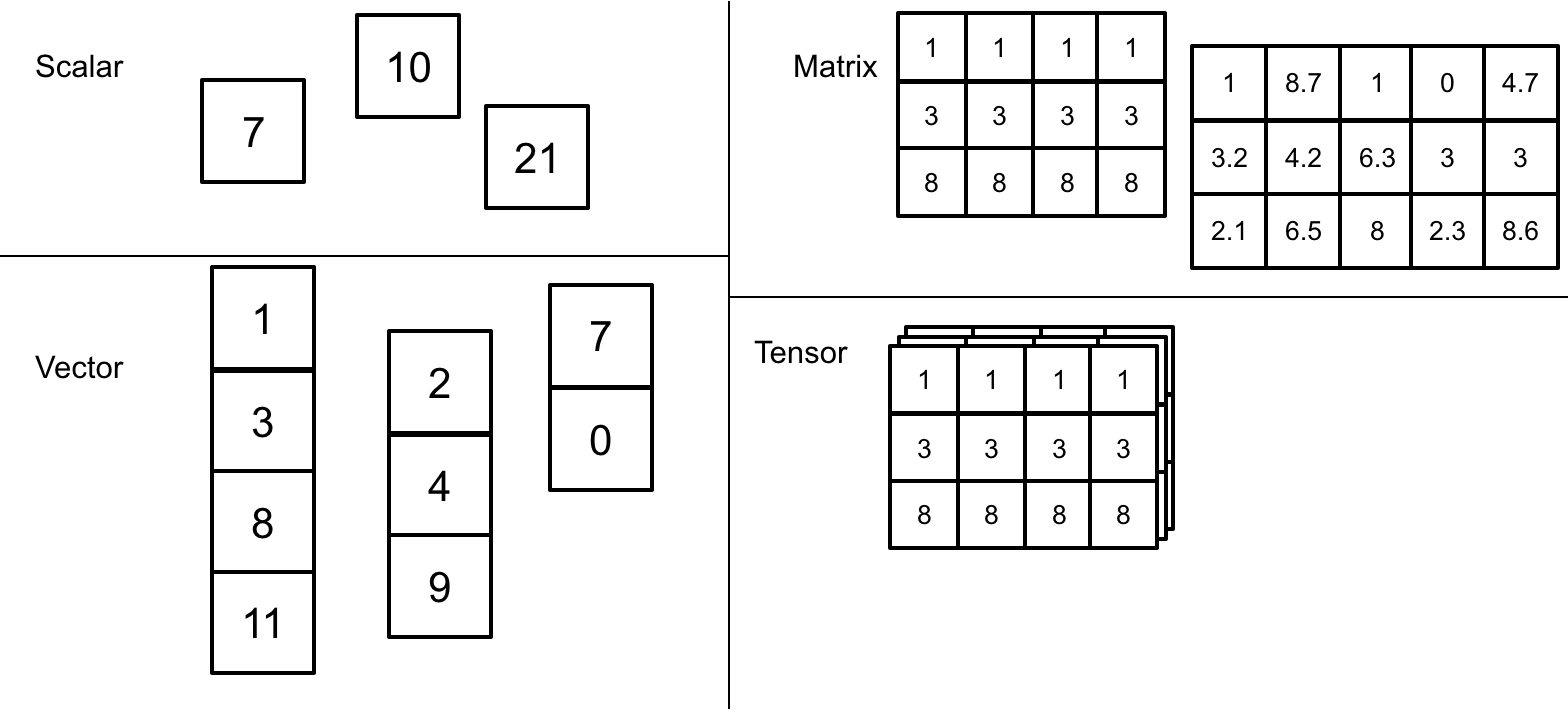
\includegraphics[scale=0.3]{img/tensor.png}
    \end{center}
    \caption{Một số khái niệm trong TensorFlow \cite{tensor}}
    \label{refhinh22}
    \end{figure}
\end{center}